\chapter{Классификация существующих решений (методов решения, алгоритмов)}

Описываются существующие решения, даются ссылки. Предлагаются критерии оценки методов. Хорошо, если критерии имеют обоснование. Приводится классификация решений по критериям в виде таблицы, но в отдельных случаях можно и не в виде таблицы (пример мы Вам кидаем отдельно от документа).

В данном разделе описываются существующие решения задчи упрощения текстов, предлагаются критерии оценки методов и приводится классификация решений по этим критериям.

\section{Существующие подходы}

Глобально выделяют два подхода к решению задачи упрощения текстов - экстрактивный (извлекающий) и абстрактный.

Большинство ранних работ, посвященных задаче упрощения текстов, использовали экстрактивный подход - выделение в документе тех предложений, которые передают больше информации. Этот подход достаточно прост в реализации, однако он подходит лишь для решения задачи упрощения текстов в широком смысле, поэтому в дальнейшем в данной работе рассматриваться не будет.

С ростом доступности вычислительных ресурсов и количества исследований в области NLP для решения задачи упрощения текстов все чаще стал использоваться абстрактный подход, подразумевающий генерацию нового текста \cite{see_get_2017}. 

\section{Решения абстрактного подхода}

Решения задачи упрощения текстов, относяшиеся к абстрактному подходу, можно разделить на решения в виде лексического упрощения и в виде генерации нового текста.

Первоначально абстрактный подход подразумевал упрощение предложений за счет лексических замен на уровне слов или целых фраз \cite{paetzold_survey_2017}. Этот процесс фокусируется исключительно на сокращении лексического содержания текста, но не принимает во внимание такие подзадачи, как грамматическое или синтаксическое упрощение \cite{shardlow_survey_2014}. Таким образом, эти решения не учитывают все аспекты решаемой задачи и поэтому в дальнейшем в работе рассматриваться не будут.

Современные решения, основанные на абстрактном подходе,  включают в себя разбиение сложных предложений на более простые, удаление редко употребляемых слов и генерацию на этой основе нового текста. Это стало возможным благодаря появлению нейронных сетей, в частности, рекуррентных нейронных сетей (RNNs)\footnote{Рекуррентная нейронная сеть, или RNN, - это сеть, которая работает с последовательностью и использут собственные промежуточные выходные данные в качестве входных данных для последующих шагов \cite{noauthor_nlp_nodate}}, которые позволяют решать задачи <<от последовательности к последовательности>> (seq2seq)\footnote{Сеть sequence-to-sequence (<<от последовательности к последовательсности>>), или сеть seq2seq, или сеть кодировщика-декодера, представляет собой модель, состоящую из двух RNN, называемых кодировщиком и декодером. Кодер считывает входную последовательность и выдает один вектор, а декодер считывает этот вектор для создания выходной последовательности \cite{noauthor_nlp_nodate}}.

Последовательность действий в решении задач, сведенных к seq2seq, является универсальной. Предварительная обработка данных включает очистку входного и результирующего текста, удаление знаков препинания и специальных символов, формирование словаря типичных слов. Далее входные и результирующие предложения преобразовываются в числовую форму с вектором одинаковой длины либо путем их усечения, либо путем их дополнения. Затем модель обучаетсяя, после чего новые поступающие данные также сначала векторизуются, преобразуются к определенной длине и упрощаются, а только после этого преобразовываются обратно из числовой формы в текстовую.


\section{Генерация нового текста}

Далее будут рассмотрены различные виды решений задачи упрощения текста, относящиеся к классу тех, которые используют генерацию нового текста.

\subsection{Синтаксическое упрощение}

Цель синтаксического упрощения заключается в выявлении грамматически сложных частей текста и их переписывание для облегчения понимания. Такое упрощение может включать разделение длинных предложений на более короткие фрагменты, переписывание предложений со страдательным залогом так, чтобы в них использовался залог действительный\footnotemark{}, разрешение двусмысленностей и анафор \cite{shardlow_survey_2014}. По ходу выполнения синтаксического упрощения удается заменять слова, которые являются сложными из-за наложения морфем, участвующих в переводе слова из одной части речи в другую, на их более простые, оригинальные версии.

\footnotetext{
Действительный залог имеют глаголы переходные, обозначающие действие, производимое субъектом и активно направленное на объект. Действительный залог имеет синтаксическую характеристику: субъект действия является подлежащим, а объект - дополнением в винительном падеже без предлога: Мир победит войну.

Страдательный залог выражается присоединением к глаголам действительного залога аффикса -ся (ср.: Рабочие строят дома. - Дома строятся рабочими). Кроме того, значение страдательного залога может быть выражено формами страдательных причастий - полных и кратких. Например: Мать любима (любимая). Тема изучена (изученная)\cite{rus_pas}.
}

Основополагающей работой в области синтаксического упрощения была система автоматического создания правил переписывания предложений \cite{chandrasekar_automatic_1997}, которая брала аннотированные корпуса и изучала возможные принципы упрощения для конкретной предметной области.  

Более поздние работы по синтаксическому упрощению были сосредоточены на улучшении структуры выходного текста - обеспечении того, чтобы предложения появлялись в правильном порядке \cite{siddharthan_syntactic_2006}. Также этот подход стали использовать для распознавания именованных сущностей (Named Entity Recognition, NER), особенно в области медицины \cite{jonnalagadda_biosimplify_2010}.

Синтаксическое упрощение обычно выполняется в три этапа. Пример применения каждого этапа к предложению показан на рисунке \ref{fig:3steps}

\begin{figure}[h!]
	
	\centering{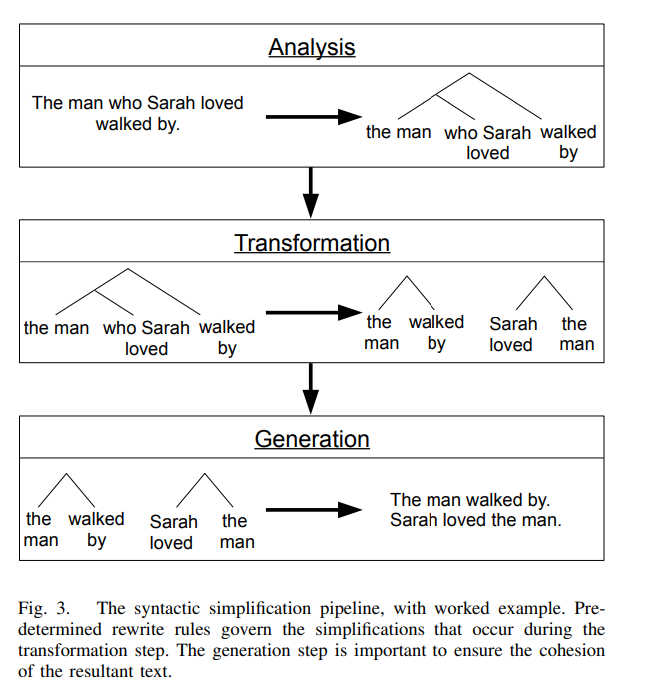
\includegraphics[scale=1]{inc/img/3steps.png}}
	
	\caption{todo}
	
	\label{fig:3steps}
	
\end{figure}

\begin{enumerate}
	\item Сначала текст анализируется для определения его структуры и создания дерева синтаксического анализа. Это может быть сделано на разных уровнях детализации, но наилучшие результаты достигаются на довольно грубом уровне, когда слова и фразы группируются в так называемые <<супер-теги>>, представляющие собой фрагменты исходного предложения. Такие теги могут быть объединены по обычным грамматическими правилами и являются структурированной версией текста. На этом же этапе простой проверкой по заранее заданным правилам или с помощью бинарного классификатора SVM\footnotemark{} \cite{shardlow_survey_2014} определяется сложность предложения.
	\footnotetext{<<Машина опорных векторов>> (Support Vector Machine, SVM) - это алгоритм машинного обучения с учителем, который в основном используется в задачах классификации. Каждая запись представляется в виде точки в n-мерном пространстве (где n - количество признаков), при этом значение каждого признака равно значению определенной координаты. Затем выполняется классификацию, в результате которой находится гиперплоскость, разделяющая два класса \cite{noauthor_svm_2017}.}
	
	\item На этапе преобразования дерево синтаксического анализа модифицируется в соответствии с набором правил, которые выполняют операции упрощения. Например, разбиение сложного предложения на более простые, перестановка или удаление этих простых предложений\cite{hutchison_ernesta_2013}.
	
	\item Далее следует фаза восстановления предложения, в ходе которой в текст вносятся дополнительные изменения для улучшения согласованности и удобства чтения.
\end{enumerate}

Синтаксическое упрощение считалось важным компонентом систем упрощения текстов и было реализовано в системах, которые повсеместно используются как вспомогательные, например, в PSET\cite{alva-manchego_data-driven_2020alva-manchego_data-driven_2020} и Porsimples\cite{aluisio_fostering_2010}.

Преимущества синтаксического упрощения заключаются в его высокой точности и применимости к другим задачам NLP \cite{shardlow_survey_2014}. Недостатком является трудоемкость создания и проверки применимости правил перезаписи. В последнее время достижения в области методов глубокого обучения привели к автоматизации процесса обнаружения возможности применения синтаксического упрощения.


\subsection{Статистический машинный перевод}
Автоматизированный машинный перевод является устоявшейся техникой в NLP. Эта задача подразумевает автоматическое преобразование лексики и синтаксиса одного языка в синтаксис другого, в результате чего получается переведенный текст. Машинный перевод был успешно применен\cite{shardlow_survey_2014} к задаче упрощения текстов путем ее переформулирования в задачу <<одноязычного перевода>>. То есть задача упрощения сводится к переводу с исходного <<сложного>> русского языка на целевой <<простой>> русский язык.

Разновидностью машинного перевода является статистический машинный перевод (Statistical Machine Translation (SMT)), основанный на статических моделях, которые изначально <<ничего не знают о правилах и лингвистике>>, а затем изучают большие объемы пар предложений из выровненных двуязычных корпусов, настраивая свои параметры (наиболее вероятный вариант перевода того или иного слова), а затем применяются к новым текстам. 

Например, модель для перевода с русского на английский изучила перевод одного предложения: <<Я вижу дом>> в <<I see a house>>. Если теперь запросить у нее перевод слова <<дом>>, она предположит, что слово с равной вероятностью переводится как <<I>>, <<see>>, <<a>> или <<house>>. Но если предоставить модели еще одно соответствие, что предложение <<Этот дом большой>> переводится как <<That house is big>>, то из анализа уже двух сопоставлений переводчик отметит, что в переводах все слова встретились по одному разу, а <<house>> — дважды, равно как и слово <<дом>> (и никакое другое) в исходных предложениях. А значит, по сравнению со всеми остальными вариантами увеличивается вероятность соответствия <<дом = house>> и между ними установилась связь. 

Данная задача облегчается, когда исходный и целевой языки схожи, и для перевода предложений требуется минимальное число изменений его структуры. И именно этот тип машинного перевода был применен к задаче упрощения текстов\cite{shardlow_survey_2014}.

%Практически системы часто используют и модифицируют стандартный инструмент SMT, такой как Moses [43], который был применен к задаче TS для английского языка [20]. Мозес был дополнен модулем удаления фраз, который удалял ненужные части сложного исходного текста с многообещающими результатами [76].


Эффективность применения статического машинного перевода для задачи упрощения предложений в значительной степени зависит от набора данных, используемых для обучения модели. Например, если в них содержатся слишком длинные исходные предложения или упрощененные предложения слишком сильно оличаются по своей структуре от входных, то этот подход не позволит отслеживать и верно сопоставлять различные части предложений. Кроме того, данный метод не учитывает знаки препинания и разбиение сложных предложений, что прииводит к потере основного контекста.


\subsection{Использование методов глубокого обучения}

Глубокое обучение - это разновидность машинного обучения, в которой нейронные сети и алгоритмы, основанные на структуре и функционировании человеческого мозга, обучаются на большом объеме данных для создания шаблонов принятия решений. Этот подход позволяет обучаться путем многократного выполнения задач и настройки модели для улучшения результата\cite{deep}.

Методы глубокого обучения после своего появления стали активно применяться для решения задачи упрощения текстов, сформулированной в терминах моделирования seq2seq. Однако в ранних моделях seq2seq были две существенные проблемы.

Во-первых, это неточность результата. Эффективность моделей кодировщика-декодера сильно зависит от расположения слов в исходном предложени, поэтому модель зачастую не может расположить редко употребляемые слова в корректную позицию выходного предложения. Один из вариантов решения этой проблемы -   добавление <<указателя>> на подобные слова в исходном тексте\cite{nisioi_exploring_2017}. Такое решение показало многообещающие результаты в сохранении точного контекста сгенерированного упрощенного текста.

Во-вторых, это повторения в выводе. Данная проблема часто возникает в простых моделях seq2seq из-за того, что так называемые <<стоп-слова>> (<<как>>, <<и>>, <<а>>, <<то>> и т. д.) встречаются в тексте намного чаще остальных, и модель учится чаще предсказывать эти слова. В частности, именно эта проблема стала основным недостатком в решении, описанном ранее\cite{nisioi_exploring_2017}. Для борьбы с этим недостатком было предложено штрафовать модель за повторения с помощью введение векторов <<покрытия>>, <<внимания>> и <<контекста>>. Эти вектора отслеживают слова, которые передаются из исходного предложения в упрощенное: вектор <<внимания>> - слова, несущие основной смысл, <<контекста>> - сопуствующую информацию, <<покрытия>> - общий переданный объем слов. Именно вектор покрытия призван дополнительно контроллировать вектора  <<внимания>> и <<контекста>> и штрафовать модель при их наложении друг на друга\cite{see_get_2017}.

Также к задаче упрощенияя текстов была успешно применена техника обучения с подкреплением\cite{zhang_sentence_2017}. Была разработана модель кодировщика-декодера в сочетании с системой глубокого обучения с подкреплением DRESS (сокр. от Deep Reinforcement Sentence Simplification, глубокое упрощение предложений с подкреплением), стремящаяся оптимизировать функцию потерь, которая поощряет простые, легко читаемые и сохраняющие исходный смыл результаты упрощения. С помощью этой модели было показано, что обучение с подкреплением предоставляет возможномть для предоставления дополнительной (предварительной) информации в данные. 

%Так, модель кодера-декодера LSTM была успешна применена\cite{wang_experimental_2016} для обучения таким операциям, как реверсирование, сортировка и замена из пар последовательностей, которые аналогичны правилам упрощения, изменяющим структуру предложения, заменяющим и удаляющим слова.

Все топовые модели использовали ту или иную форму фильтрации обучающего набора данных или обработки управляющих маркеров и тонкой настройки крупномасштабных предварительно обученных языковых моделей. Выигрышное решение (qbic) в значительной степени основано на упрощении многоязычных предложений без присмотра [16]. Модель состоит из MBART[19], точно настроенной на Paraphraserplus[9] и RuWikiSimple, основанной на определенных контрольных маркерах (сходство Левенштейна, доля совпадающих символов между оригинальными и упрощенными предложениями, ранг слова, сходство лексем). Несколько других моделей, занявших первое место (оржан, занявший второе место, ашатилов, занявший третье место, и аленуш, занявший пятое место ), являются генеративными (модели на основе GPT), точно настроенными на отфильтрованном примере RuWikiSimple. Чтобы быть более конкретным, второй-помещается модель orzhan является ruGPT-3 доработаны на RSSE Дев набора и фильтруют RuWikiSimple, где фильтрация проводилась с помощью 6 различных метрик (предложении встраивание Косинус сходство, именованных сущностей результат сохранения, лексических результат сложности, зависимость глубина дереве счет, счет длины и чтения). Выбор лучшего кандидата из предложенных вариантов сгенерированный моделью путем оптимизации комбинации этих шести показателей вместо SARI, учитываемых для Улучшение на 0,6 САРИ в частном тесте.

Решение Ашатилова, занявшее третье место, использовало модель на основе GPT-2[13]. Как простая фильтрация Ruwik, так и выбор кандидатов выполнялись с помощью четырех показателей (косинусное сходство, ROUGE-L и длина ввода и кандидата в токенах). Однако, в отличие от модели оржана, вместо ручного объединения четырех показателей в агрегат ашатилов выбирает лучшего кандидата путем обучения классификатора случайных лесов, где в качестве признаков используются четыре показателя.

Несколько других решений на основе mBART обогащены некоторыми дополнительными функциями и технологиями. Они включали предварительную подготовку по дополнительным источникам данных (наиболее популярным из которых был ParaPhraserPlus), различные функции ручной работы и обратный перевод[26].

Анализируя результаты, можно предположить, что выбор между предварительной подготовкой seq2seq (т. е. на основе MBART) и генеративными моделями (на основе GPT) оказывает ограниченное влияние на конечный результат. Использование дополнительных показателей для фильтрации набора данных, отбора кандидатов и/или в качестве контрольных маркеров, наоборот, представляется крайне важным для дальнейшего повышения производительности. Похоже, что выбор показателей в двух лучших моделях лучше, чем те, которые используются в третьей модели. С другой стороны, обучение отдельной модели для выбора лучшего кандидата (как это делается моделью, занявшей третье место), по-видимому, приводит к меньшему переобучению, чем использование совокупной метрики с фиксированными параметрами (о чем свидетельствует сокращение модели ашатилова на 0,4 САРИ по сравнению с моделью Ашатилова до 1 САРИ оржана и аленуша). Для подтверждения этих утверждений необходимо провести дополнительные исследования.

\section{Метрики}

Оценка качества упрощения текста - довольно субъективная задача, трудно переводимая на язык компьютера. Поэтому до сих пор предпочтение отдается человеку, который оценивает упрощенное предложение с точки зрения его грамматической корректности, сохранения смысла и простоты, используя шкалы Лайкерта\footnotemark{}. Однако тенденция к использованию технологии обучения без учителя потребовала разработки или адаптации уже существующих показателей для автоматической оценки качества упрощения.\footnotetext{Шкала Лайкерта - это ординальная (порядковая) шкала ответов на вопрос или утверждений, расположенных в иерархической последовательности, например, от «полностью согласен» через «затрудняюсь ответить» и до «категорически не согласен»\cite{likert}.}

\subsection{SARI}

Метрика SARI (\textbf{s}ystem output \textbf{a}gainst \textbf{r}eferences and against the \textbf{i}nput sentence - результат системы против эталонного решения и исходного предложения) была разработана в 2016 году специально для задачи упрошения и в настоящее время считается наиболее применимой\cite{xu_optimizing_2016}.

Авторы SARI заметили, что в отличие от метрик качества машинного перевода, где исходное предложение записано на другом языке, метрики качества упрощения могут использовать еще один источник для оценки результирующего предложения - само исходное предложение, так как оно записано на том же языке, что и упрощенное. Разработанная ими метрика явно оценивает, насколько корректно были выбраны слова, которые были добавлены, удалены или же сохранены моделью.

Результаты исследования аворов показали высокую корреляцию оценки метрикой SARI с оценками качества упрощения человеком, однако , эта функция требует нескольких <<справочных>> примеров упрощения, которые не всегда доступны.

\subsection{Индексы удобочитаемости}
Индексы удобочитаемости используются в США для присвоения любому тексту уровня его <<простоты>>. Обычно для такой оценки применяется сразу несколько формул, которые учитывают количество предложений, слогов, общее количество слов и количество редких слов в рассматриваемом тексте. Отличаются эти формулы лишь коэффициентами, расположением членов в формуле или способом интерпретации результата.

Например, в тесте Флэша-Кинкайда предполагается, что чем меньше слов в предложениях и чем короче слова, тем более простым является текст. В результате применения формулы \ref{eq:1} корпус получает оценку, по которой с помощью специальной таблицы интерпретируется уровень образования, необходимый для понимания текста\cite{test}.

\begin{eqnarray} 
	\label{eq:1}
	206.835 - 1.015 \cdot \left(\frac{\textrm{количество слов}}{\textrm{количество предложений}}\right) - \notag\\ - 84.6 \cdot \left(\frac{\textrm{количество слогов}}{\textrm{количество слов}}\right) 
\end{eqnarray}


Основной недостаток индексов удобочитаемости заключается в том, что используемые в них формулы <<поощеряют>> короткие предложения с простыми словами, но не способны распознавать грамматически неправильные результаты или упрощенные предложения, некорректно передающие смысл исходного.

– SAMSA - A new metric proposed by Sulem et al. that can evaluate simplification, including
sentence splitting, not just summarization, like SARI [89]. Due to its recent release, this
metric is not currently widely used.

